\section{Test on toy model}
This section creates two toy models to test the data reconstruction and model comparison ability of the network.

Model 1,
$$
\begin{aligned}
&y=A z^{2}+(-A+B) z+C \\
&\text { where, } A \sim \mathcal{N}(-4,0.1), B \sim \mathcal{N}(0,0.01), C \sim \mathcal{N}(0,0.1)
\end{aligned}
$$
Model 2,
$$
\begin{aligned}
&y=A \sin (\omega z)+C \\
&\text { where, } A \sim \mathcal{N}(1,0.1), \omega \sim \mathcal{N}(\pi, 0.01), C \sim \mathcal{N}(0,0.1)
\end{aligned}
$$

Model 1 and Model 2 have similar distributions as shown in Figure 2 Given the observations $\boldsymbol{x}_{\text {obs,real }}$ which are generated by the underlying model $y_{\text {true }}=-3.5 z^{2}+3.6 z-0.1$ on $\boldsymbol{z}_{\text {obs }}=\left\{z_{1}, z_{2}, \cdots, z_{580}\right\}$ with an error matrix $\Sigma_{o b s}$, we would like to fit the two toy models to the observations to tell which one is most probable to be the true model, and interpolate the data with the model at $\boldsymbol{z}^{*}=\left\{z_{1}^{*}, \cdots, z_{M}^{*}\right\}$, for example, $\boldsymbol{z}^{*}$ even staying in the interval $[0,1]$ with $M=1468$.

\begin{figure}
	\centering
	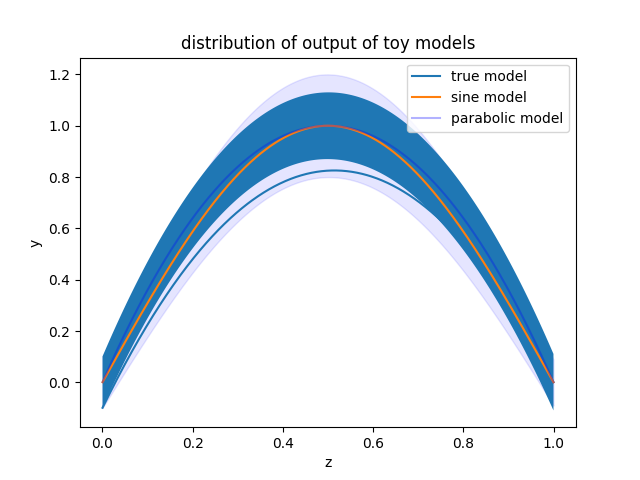
\includegraphics[width=\textwidth]{toy/dist_toy_models.png}
	\caption{Toy models}
	\label{fig:toy_model}
\end{figure}

First we concatenate and sort $\boldsymbol{z}$ and $\boldsymbol{z}^{*}$, and call the new one $\boldsymbol{z}$. Then sample $\left\{A_{i}, B_{i}, C_{i}, \omega_{i}\right\}$ from the priors of the toy models and generate the training samples $\boldsymbol{x}_{i}=M_{k}\left(\boldsymbol{z} \mid A_{i}, B_{i}, C_{i}, \omega_{i}\right.$ ) (Note that which set of parameters should be used depends on the toy model). Here 12800 samples for each model are generated as the training dataset. Finally, the training set $\{\boldsymbol{x}\}_{i=1}^{25600}$ together with the observation error $\Sigma_{o b s}$ is fed into the network. Once the training converges, one can put the observations $\boldsymbol{x}_{o b s, r e a l}$ into the network to tell which toy model is most probable and get the interpolation, see Figure 3 In this task, the discriminator has a classification accuracy of almost 1. It assigns a probability of $97 \%$ to the parabolic model (Model 1), which is indeed the case.

\begin{figure}
	\centering
	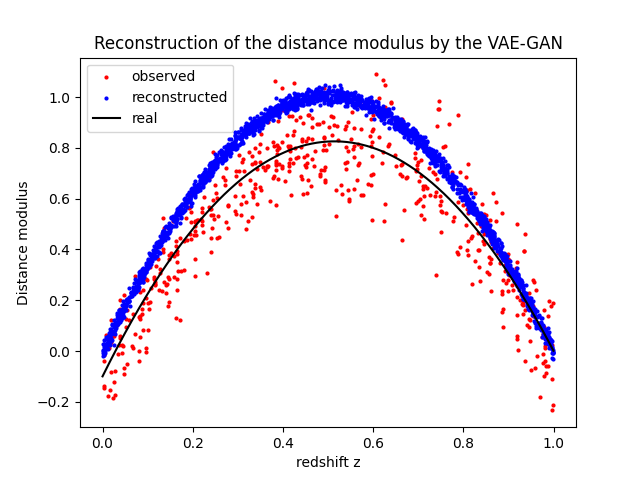
\includegraphics[width=\textwidth]{toy/true_vs_reconstructed.png}
	\caption{Reconstruction}
	\label{fig:recon_toy}
\end{figure}